%% AMS-LaTeX Created by Wolfram Mathematica 9.0 : www.wolfram.com

\documentclass[DIV12]{scrartcl}
\usepackage{amsmath, amssymb, graphics, setspace}

\newcommand{\mathsym}[1]{{}}
\newcommand{\unicode}[1]{{}}

\newcounter{mathematicapage}

\title{Physikbasierte Modellierung und Simulation}
\author{}
\date{}

\begin{document}

\maketitle

\section*{Aufgabe 9.1}

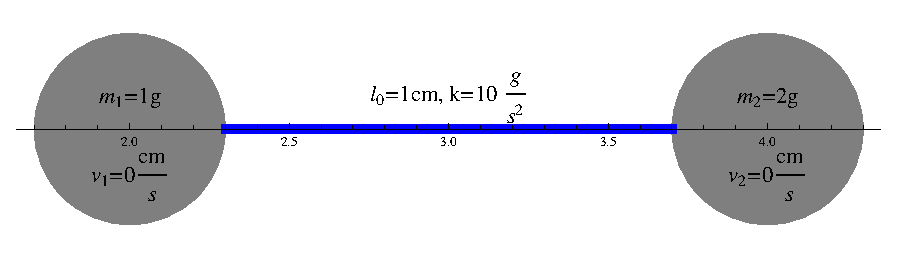
\includegraphics{ex09_gr1.eps}


\section*{Aufgabe 9.2}

Hooke{'}s Gesetz: \(F=k\left(l_0-l\right)\) mit Betrachtung der Richtung der Kraft:
\\\\
\(\Rightarrow  F_1=k(l_0-| x_1-x_2| )\cdot\frac{x_1-x_2}{| x_1-x_2| }=10\frac{g}{s^2}(1\text{cm}-|
2\text{cm}-4\text{cm}| )\cdot\frac{2\text{cm}-4\text{cm}}{| 2\text{cm}-4\text{cm}| }=10\frac{g}{s^2}(-1\text{cm})\cdot(-1)=10\text{cm} \frac{g}{s^2}\)\\
\(\Rightarrow  F_2=k(l_0-| x_2-x_1| )\cdot\frac{x_2-x_1}{| x_2-x_1| }=10\frac{g}{s^2}(1\text{cm}-|
4\text{cm}-2\text{cm}| )\cdot\frac{4\text{cm}-2\text{cm}}{| 4\text{cm}-2\text{cm}| }=10\frac{g}{s^2}(-1\text{cm})\cdot1=-10\text{cm} \frac{g}{s^2}\)

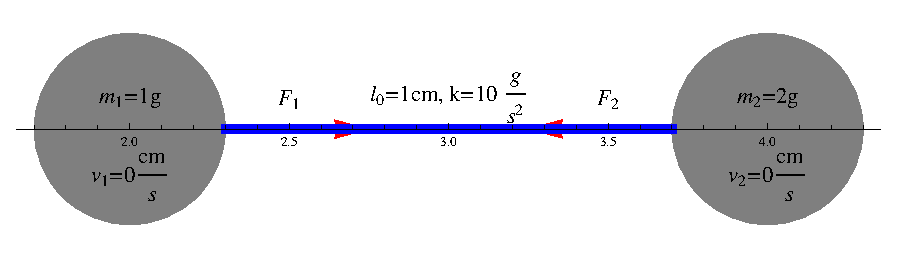
\includegraphics{ex09_gr2.eps}

\section*{Aufgabe 9.3}

\(x_1(t+h)=x_1(t)+h x_1'(t)=x_1(t)+h v_1(t)=2\text{cm} +1 s \cdot 0\frac{\text{cm}}{s}=2\text{cm}\)\\
\(x_2(t+h)=x_2(t)+h x_2'(t)=x_2(t)+h v_2(t)=4\text{cm} +1 s \cdot 0\frac{\text{cm}}{s}=4\text{cm}\)
\\\\
\(a_1(t)=\frac{F_1}{m_1}=\frac{10\text{cm} \cdot g}{s^2\cdot1 g}=10 \frac{\text{cm}}{s^2}\)\\
\(a_2(t)=\frac{F_2}{m_2}=\frac{-10\text{cm} \cdot g}{s^2\cdot2 g}=-5 \frac{\text{cm}}{s^2}\)
\\\\
\(v_1(t+h)=v_1(t)+h v_1'(t)=v_1(t)+h a_1(t)=0\frac{\text{cm}}{s}+1s\cdot10\frac{\text{cm}}{s^2}=10\frac{\text{cm}}{s}\)\\
\(v_2(t+h)=v_2(t)+h v_2'(t)=v_2(t)+h a_2(t)=0\frac{\text{cm}}{s}+1s\cdot-5\frac{\text{cm}}{s^2}=-5\frac{\text{cm}}{s}\)
\\\\
Nicht stabil, da sich im n{\" a}chsten Schritt beide Kugeln durchdringen werden; kausal nicht erkl{\" a}rbar.

\section*{Aufgabe 9.4}

\begin{itemize}
    \item[a)]

        Da hier auf jeden Fall: \(x_2>x_1\) gilt, k{\" o}nnen \(F_1\) und \(F_2\) wie folgt vereinfacht werden:

        \(F_1\left(x_1, x_2\right)=k\left(l_0-\left(-\left(x_1-x_2\right)\right)\right)\cdot\frac{x_1-x_2}{-\left(x_1-x_2\right)}=-k\left(l_0+x_1-x_2\right)\)\\
        \(F_2\left(x_1, x_2\right)=k\left(l_0-\left(x_2-x_1\right)\right)\cdot\frac{x_2-x_1}{x_2-x_1}=k\left(l_0+x_1-x_2\right)\)

        Damit ist die Jakobi-Matrix:
        \(J=\left(
        \begin{array}{cc}
         \frac{\partial F_1}{\partial x_1} & \frac{\partial F_1}{\partial x_2} \\
         \frac{\partial F_2}{\partial x_1} & \frac{\partial F_2}{\partial x_2} \\
        \end{array}
        \right)=\left(
        \begin{array}{cc}
         -k & k \\
         k & -k \\
        \end{array}
        \right)\)

    \item[b)]

    \(\left(
    \begin{array}{c}
     m_1a_1' \\
     m_2a_2' \\
    \end{array}
    \right)=\left(
    \begin{array}{c}
     F_1 \\
     F_2 \\
    \end{array}
    \right)+h J \left(
    \begin{array}{c}
     v_1 \\
     v_2 \\
    \end{array}
    \right)+h^2 J \left(
    \begin{array}{c}
     a_1' \\
     a_2' \\
    \end{array}
    \right)=\left(
    \begin{array}{c}
     10 \\
     -10 \\
    \end{array}
    \right)\text{cm}\frac{g}{s^2}+ 1 s \cdot \left(
    \begin{array}{cc}
     -10 & 10 \\
     10 & -10 \\
    \end{array}
    \right) \frac{g}{s^2}\cdot\left(
    \begin{array}{c}
     0 \\
     0 \\
    \end{array}
    \right)\frac{\text{cm}}{s}+ (1s)^2\cdot\left(
    \begin{array}{cc}
     -10 & 10 \\
     10 & -10 \\
    \end{array}
    \right) \frac{g}{s^2}\left(
    \begin{array}{c}
     a_1' \\
     a_2' \\
    \end{array}
    \right) \Leftrightarrow\)
    \\\\\\
    \(\left(
    \begin{array}{cc}
     1 & 0 \\
     0 & 2 \\
    \end{array}
    \right)\left(
    \begin{array}{c}
     a_1' \\
     a_2' \\
    \end{array}
    \right)g=\left(
    \begin{array}{c}
     10 \\
     -10 \\
    \end{array}
    \right)\text{cm}\frac{g}{s^2}+\left(
    \begin{array}{cc}
     -10 & 10 \\
     10 & -10 \\
    \end{array}
    \right) \left(
    \begin{array}{c}
     a_1' \\
     a_2' \\
    \end{array}
\right)g\)
\(\Leftrightarrow\)
    \\\\\\
    \(\left(
    \begin{array}{c}
     10 \\
     -10 \\
    \end{array}
    \right)\frac{\text{cm}}{s^2}=\left(
    \begin{array}{cc}
     11 & -10 \\
     -10 & 12 \\
    \end{array}
    \right)\left(
    \begin{array}{c}
     a_1' \\
     a_2' \\
    \end{array}
    \right) \Leftrightarrow\)
    \\\\\\
    \(\left(
    \begin{array}{c}
     a_1' \\
     a_2' \\
    \end{array}
    \right)=\left(
    \begin{array}{cc}
     \frac{3}{8} & \frac{5}{16} \\
     \frac{5}{16} & \frac{11}{32} \\
    \end{array}
    \right)\left(
    \begin{array}{c}
     10 \\
     -10 \\
    \end{array}
    \right)\frac{\text{cm}}{s^2} \Leftrightarrow\)
    \\\\\\
    \(\left(
    \begin{array}{c}
     a_1' \\
     a_2' \\
    \end{array}
    \right)=\left(
    \begin{array}{c}
     \frac{5}{8} \\
     -\frac{5}{16} \\
    \end{array}
    \right)\frac{\text{cm}}{s^2}\)

    \item[c)]

        \(\left(
        \begin{array}{c}
         v_1' \\
         v_2' \\
        \end{array}
        \right)=\left(
        \begin{array}{c}
         v_1 \\
         v_2 \\
        \end{array}
        \right)+h\left(
        \begin{array}{c}
         a_1' \\
         a_2' \\
        \end{array}
        \right)=\left(
        \begin{array}{c}
         0 \\
         0 \\
        \end{array}
        \right)\frac{\text{cm}}{s}+1s\cdot\left(
        \begin{array}{c}
         \frac{5}{8} \\
         -\frac{5}{16} \\
        \end{array}
        \right)\frac{\text{cm}}{s^2}=\left(
        \begin{array}{c}
         \frac{5}{8} \\
         -\frac{5}{16} \\
        \end{array}
        \right)\frac{\text{cm}}{s}\)
        \\\\
        \(\left(
        \begin{array}{c}
         x_1' \\
         x_2' \\
        \end{array}
        \right)=\left(
        \begin{array}{c}
         x_1 \\
         x_2 \\
        \end{array}
        \right)+h\left(
        \begin{array}{c}
         v_1' \\
         v_2' \\
        \end{array}
        \right)=\left(
        \begin{array}{c}
         2 \\
         4 \\
        \end{array}
        \right)\text{cm}+1s\cdot\left(
        \begin{array}{c}
         \frac{5}{8} \\
         -\frac{5}{16} \\
        \end{array}
        \right)\frac{\text{cm}}{s}=\left(
        \begin{array}{c}
         \frac{21}{8} \\
         \frac{59}{16} \\
        \end{array}
        \right)\text{cm}=\left(
        \begin{array}{c}
         2.625 \\
         3.6875 \\
        \end{array}
        \right)\text{cm}\)
        \\\\
        Die Beschleunigung ist hier weniger extrem, was zu glaubw\"urdigeren Positionen und einer stabileren Simulation f\"uhrt.
\end{itemize}

\end{document}
